

\begin{asm}
  \label{asm:surfaceForceViscous}
  From now on, 
  assume that
  \begin{equation}
    \label{equ:surfaceForceSigma}
    \text{force on $S$ per unit area} = -p(\mathbf{x}, t)\mathbf{n}+\mathbf{n}\cdot\boldsymbol\sigma(\mathbf{x}, t), 
  \end{equation}
  where $\boldsymbol\sigma$ is the \emph{(deviatoric) stress tensor} and
  $\mathbf{n}$ is the unit outward normal of $S$.
\end{asm}

%%% Local Variables:
%%% mode: latex
%%% TeX-master: "../notesOnFluidMechanics"
%%% End:
\newpage
\section{Spike-Train Statistics}
\label{sec:1.4}


\begin{rem}
        A complete description of the stochastic relationship between a stimulus and a response would require us to know the probabilities corresponding to every sequence of spikes that can be evoked by the stimulus.    
\end{rem}

\begin{lem}
    The probability that $z$ takes a value between $z$ and $z+ \Delta z$, for small $\Delta$(strictly speaking, as $\Delta z \to 0$), is equal to $p[z]\Delta z$, where $p[z]$ is called a probability density.
\end{lem}

\begin{ntn}    
    Throughout this book,  we use the notation $P$[\ ] to denote probabilities and $p$[\ ] to denote probability densities.
\end{ntn}    


\begin{thm}
    The probability of a spike sequence appearing is proportional to the probability density of spike times,  $p[t_1, t_2, ..., t_n]$. In other words, the probability $P[t_1,t_2,...,t_n]$ that a sequence of n spikes occurs with spike $i$ falling between times $t_i$ and $t_i+\Delta t$ for $i= $1,2,...,n is given in terms of this density by the relation 
    \begin{equation}
        P[t_1,t_2,...,t_n]=p[t_1,t_2,...,t_n](\Delta t)^n.        
    \end{equation}
    % This relationship is a special case of Equation \ref{equ:1.37} derived below.
    \begin{proof}
        \small
        $$P[t_1,t_2,...,t_n]=\int... \int p[s_1,s_2,...,s_n]dS\\$$
        $$=\int^{t_n+\Delta t/2}_{t_n-\Delta t/2} 
        \int^{t_{n-1}+\Delta t/2}_{t_{n-1}-\Delta t/2} ...\int^{t_1+\Delta t/2}_{t_1-\Delta t/2} p[s_1,s_2,...,s_n]ds_1 ...ds_{n-1}ds_{n}\\$$
  \\ According to the integral mean value theorem ( $\Delta t \to 0  $ )\\
        $\Rightarrow  P[t_1,t_2,...,t_n]=p[t_1,t_2,...,t_n](\Delta t)^n.        $
        
    \end{proof}
\end{thm}

\begin{defn}[\emph{point process}]
    A stochastic process that generates a sequence of events, such as action potentials ,is called a point process.     
\end{defn}

\begin{rem}
    In general, the probability of an event occurring at any given time could depend on the entire history of preceding events. 
\end{rem}

\begin{defn}[\emph{renewal process}]
    If this dependence extends only to the immediately preceding event, so that the intervals between successive events are independent, the point process is called a renewal process.
\end{defn}

\begin{defn}
    The Poisson process provides an extremely useful approximation of stochastic neuronal firing.
    To make the presentation easier to follow, we separate two cases, the homogeneous Poisson process, for which the firing rate is constant over time, and the inhomogeneous Poisson process, which involves a time-dependent firing rate.
\end{defn}

\subsection{The Homogeneous Poisson Process}

\begin{ntn}
    We denote the firing rate for a homogeneous Poisson process by r$(t)=$r, because it is independent of time.
\end{ntn}

\begin{defn}[\emph{probality of $n$ spikes occuring}]
     The probality that an arbitrary sequence of exactly $n$ spikes occurs within a trial of duration $T$ is $P_T[n]$.
\end{defn}

\begin{thm}
    For a homogeneous Poisson process, the Poisson distribution is 
    \begin{equation}
        P_T[n]=\frac{(rn)^n}{n}exp(-rT).
        \label{equ:1.29}
    \end{equation}
    \begin{proof}
        To compute $P_T[n]$, we divide the time T into M bins of size $\Delta t =T/M$. We assume that $\Delta t$ is small enough so that we never get two spikes within any one bin because, at the end of the calculation,we take the limit $\Delta t \to 0$.\\
        $P_T[n]$ is the product of three factors: \\
            (a)\ The probability of generating $n$ spikes within a  specified set of the $M$ bins,$\frac{M!}{(M-n)!n!}$;\\
            (b)\ The probability of not generating spikes in the remaining $M - n$ bins,$(r\Delta t)^n$;\\
            (c)\ A combinatorial factor equal to the number of ways of putting $n$ spikes into $M$ bins,$(1-r\Delta t)^{M-n}$; \\
            \text{    To sum up,}            
            \begin{equation}
            \label{equ:1.27}
            P_T[n]=\lim_{\Delta t \to 0}\frac{M!}{(M-n)!n!}(r\Delta t)^n(1-r\Delta t)^{M-n}.
        \end{equation}
        As $\Delta t \to 0, M$ grows without bound because $ M\Delta t=T$. Because n is fixed, we can write $M-n\approx M=T/\Delta t$. Using this approximatin and defining $\epsilon=-r\Delta t$, we find that 
        \begin{equation}
            \lim_{\Delta t \to 0}(1-r\Delta t)^{M-n}=\lim_{\epsilon\to 0}(((1+\epsilon)^{\frac{1}{\epsilon}})^{-rT}=\exp(-rT)
        \end{equation}
        For large $M,\ \frac{M!}{(M-n)!}\approx M^n=(T/\Delta t)^n$, so
        \begin{equation}            
            P_T[n]=\frac{(rn)^n}{n}exp(-rT).
        \end{equation}
    \end{proof}
\end{thm}

\begin{exm}
    The probabilities $P_T[n]$, for a few $n$ values, are plotted as a function of $rT$ in the following firgue. Note that as $n$ increase, the probability reaches its maximum at larger $T$ values and that large $n$ values are more likely than small ones for large $T$.
\end{exm}    

\begin{center}
    \label{fig:1.11}                
        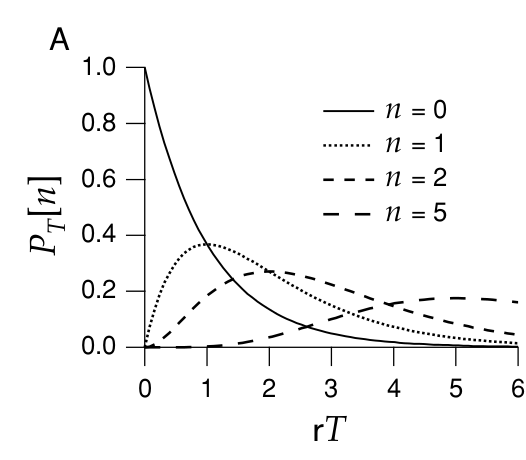
\includegraphics[scale = 0.36]{png/Figure1-11-A}\\        
\end{center}

\begin{exm}
    The following figure shows the probabilities of various numbers of spikes occurring when the average number of spikes is $10$. For large $rT$, which corresponds to a large expected number of spikes, the Poisson distribution approaches a Gaussian distribution with mean and variance equal to $rT$. This figure shows that this approximation is already quite good for $rT = 10$.
\end{exm}    

\begin{center}
    \label{fig:1.12}            
    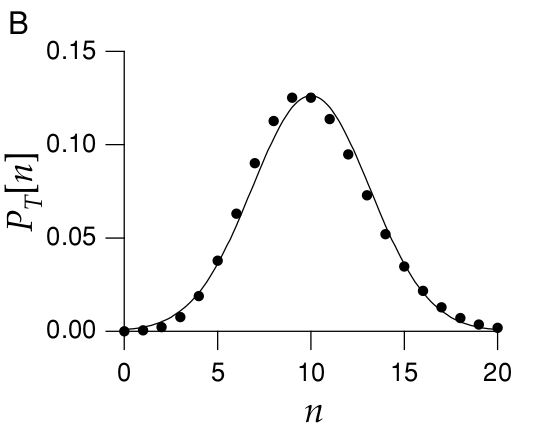
\includegraphics[scale = 0.36]{png/Figure1-11-B}\\    
\end{center}

\begin{thm}
    The probability $P[t_1,t_2,...,t_n]$ can be expressed in terms of another probability function $P_T[n]$, which is the probality that an arbitrary sequence of exactly $n$ spikes occurs within a trial of duration $T$. Assuming that the spike times are ordered $0\leq t_1\leq t_2\leq ...\leq t_n\leq T$, so that, the relationship is 
    \begin{equation}
        P[t_1,t_2,...,t_n]=n!{P_T[n]\left (\frac{\Delta t}{T}\right )^n}.
        \label{equ:1.26}
    \end{equation}
    \begin{proof}
        % represents
        The probability of docking is $ n!(\frac{\Delta t}{T})^n $ in a specific time order $(t_1,t_2,...,t_n).$  so,
       \begin{align}       
         &P[t_1,t_2,...,t_n]={P_T[n]}(n(\frac{\Delta t}{T})(n-1)(\frac{\Delta t}{T})...1(\frac{\Delta t}{T}))\\
        &=n!{P_T[n]\left(\frac{\Delta t}{T}\right)^n}
    \end{align}
    \end{proof}
\end{thm}

\begin{coro}
    We can compute the variance of spike counts produced by a Poisson process from the probabilities in Equation \ref{equ:1.29}. The spike count is 
    \begin{equation}
        \sigma^2_n = \langle n^2 \rangle -\langle n  \rangle ^2=rT.
    \end{equation}
    \begin{proof}
    The average number of spikes generated by a Poisson process with constasnt rate $r$ over a time $T$ is 
    \begin{equation}
        \langle n\rangle=\sum_{n=0}^\infty nP_T[n]=\sum_{n=0}^\infty\frac{n(rT)^n}{n!}\exp(-rT).
        \label{equ:1.45}
    \end{equation}
    and the variance in the spike count is
    \begin{equation}
        \sigma_n^2(T)=\sum_{n=0}^\infty n^2P_T[n]-\langle n\rangle^2=\sum_{n=0}^\infty\frac{n^2(rT)^n}{n!}\exp(-rT)-\langle n\rangle^2.
        \label{equ:1.46}
        \end{equation}
        To compute the quantities,we need to calculate the two sums appearing in these Equations.A good way to do this is to compute the moment-generating function
        \begin{equation}
            g(\alpha)=\sum_{n=0}^\infty\frac{(rT)^n\exp(\alpha n)}{n!}\exp(-rT).
            \label{equ:1.47}
        \end{equation}      
        The $k$th derivative of g with respect to $\alpha$,evaluated at the point $\alpha=0$, is
        \begin{equation}
            \frac{dg}{d\alpha^k}|_{\alpha=0}=\sum_{n=0}^\infty\frac{n^k(rT)^n}{n!}\exp(-rT),
            \label{equ:1.48}
        \end{equation}        
    so once we have computed $g$,we need to calculate only its first and second derivative to determine the sums we need. Rearranging the terms a bit, and recalling that $\exp(z)=\sum z^n/n!$, we find\\        
    \begin{equation}
        g(\alpha)=\exp(-rT)\sum_{n=0}^\infty\frac{(rT\exp(\alpha))^n}{n!}=\exp(-rT)\exp(rTe^\alpha).
        \label{equ:1.49}
    \end{equation}
    The derivatives are then \\
    \begin{equation}
        \frac{dg}{d\alpha}=rTe^\alpha \exp(-rT)\exp(rTe^\alpha)
        \label{equ:1.50}
    \end{equation}
    and\\
    \begin{equation}
    \small    \frac{d^g}{d\alpha^2}=(rTe^\alpha)^2\exp(-rT)\exp(rTe^\alpha)+rTe^\alpha \exp(-rT)\exp(rTe^\alpha).
        \label{equ:1.51}
    \end{equation}
    Evaluating these at $\alpha=0$and putting the results into Equation \ref{equ:1.45} and \ref{equ:1.46} gives the result $\langle n\rangle=rT$ and $$\sigma_n^2(T)=(rT)^2+rT-(rT)^2=rT.$$
    \end{proof}
\end{coro}

\begin{defn}[\emph{Fano factor}]
    % (Fano factor)The ratio of the variance and mean of the spike count ,$\sigma^2_n/\langle n\rangle$,is called the Fano factor.
    The ratio of the variance and mean of the spike count,
   $     \sigma^2_n/\langle n\rangle$, is called the Fano factor.            
\end{defn}

\begin{exm}
    The Fano factor takes the value $1$ for a homogeneous Poisson process, independent of the time interval $T$.
\end{exm}

\begin{lem}
    % For a homogeneous Poisson process,the probability of an interspike intervalfalling between $\tau$ and $\tau + \Delta t$ is $$P[\tau\leq t_{i+1}-t_{i}<\tau +\Delta t]=r\Delta t\ \exp(-r\tau)$$.
    The probability of an interspike intervalfalling between $\tau$ and $\tau + \Delta t$ is 
    \begin{equation}
        P[\tau\leq t_{i+1}-t_{i}<\tau +\Delta t]=r\Delta t\ \exp(-r\tau).
        \label{equ:1.31}
    \end{equation}
    \begin{proof}
        Suppose that a spike occurs at a time $t_i$ for some value of $i$. The probability of a homogeneous Poisson process generating the next spike somewhere in the interval $$t_i+\tau \leq t_{i+1} \leq t_i + \tau +\Delta t,$$ for small $\Delta t$, is the probabilities that no spike is fired for a time $\tau$, times the probability, $r\Delta t$, of  generating a spike within the following small interval $\Delta t$. From Equation \ref{equ:1.29}, with $n=0$, the probability of not firing a spike for period $\tau$ is $\exp(-r\tau)$. So the probability of an interspike interval falling between $\tau$ and $\tau+\Delta t$ is $$  P[\tau\leq t_{i+1}-t_{i}<\tau +\Delta t]=r\Delta t\ \exp(-r\tau).$$
    \end{proof}
\end{lem}

\begin{thm}
    From the interspike interval distribution of a homogeneous Poisson spike train,  we can compute the mean interspike interval, 
    \begin{equation}
        \langle \tau \rangle =\int^{\infty}_{0}\tau r\ \exp(-r\tau)d\tau  = \frac{1}{r}
        \label{equ:1.32}         
    \end{equation}
    and the variance of the interspike intervals, 
    \begin{equation}
        \sigma^2_\tau =\int^{\infty}_{0}\tau^2 r\ \exp(-r\tau)d\tau - \langle \tau \rangle^2 = \frac{1}{r^2}.
        \label{equ:1.33}         
    \end{equation}
\end{thm}

\begin{defn}
    % [\emph{coefficient of variation}]
    The ratio of the standard deviation and the mean of interspike interval distribution.
    \begin{equation}
        C_V=\frac{\sigma_\tau}{\langle \tau  \rangle},
        \label{equ:1.34}
    \end{equation} is the \emph{the coefficient of variation}
\end{defn}

\begin{rem}
    The coefficient of variation takes the value $1$ for a homogeneous Poisson process. This is a necessary,  though not sufficient, condition to identify a Poisson spike train. Recall that the Fano factor for a Poisson process is also $1$. For any renewal process, the Fano factor evaluated over long time intervals approaches the value $C^2_V$.
\end{rem}

\subsection{The Spike-Train Autocorrelation Funciton}

\begin{defn}
        The spike-train autocorrelation function,
        \begin{equation}
            Q_{\rho\rho}(\tau)=\frac{1}{T}\int^T_0 \langle (\rho(t)-\langle r \rangle)(\rho(t+\tau)-\langle r\rangle)\rangle dt,
            \label{equ:1.35}
        \end{equation} is the autocorrelation of the neural response function of Equation \ref{equ:1.1} with its average over time and trials substracted out. 
\end{defn}

\begin{thm}
    The autocorrelation function for a Poisson spike train generated at a constant rate $\langle r \rangle =r$ is 
    \begin{equation}
        Q_{\rho\rho}(\tau)=r\delta(\tau)
    \end{equation}
    \begin{proof}
        The spike-train auto correlation function is constructed from data in the form of a histogram by dividing time into bins. The value of the histogram for a bin labeled with a positive or negative integer $m$ is computed by determining the number of the times that any two spikes in the train are separated by a time interval lying between $(m-1/2)\Delta t$ and $(m+1/2)\Delta $ with $\Delta t$ the bin size.  This includes all pairings, even  between a spike and itself. We call this number $N_m$. If the intervals between the $n^2$ spike pairs in the train were uniformly distributed over the range from $0$ to $T$, there would be $n^2\Delta t/T$ intervals in each bin. This uniform term is removed from the autocorrelation histogram by subtracting $n^2\Delta t /T$ from $N_m$ for all $m$. The spike-train autocorrelation histogram is then defined by dividing the resulting numbers by $T$, so the value of the histogram in bin m is $H_m=N_m/T-n^2\Delta /T^2$. For small bin sizes, the $m = 0$ term in the histogram counts the average number of spikes,  that is $N_m = \langle n \rangle $ and in the limit $\Delta t \to 0,\ H_0=\langle n \rangle /T$ is the average firing rate $\langle r \rangle$. Because other bins have $H_m$ of order $\Delta t$, large $m = 0$ term is often removed from histogram plots. The spike-train autocorrlation function is defined as $H_m/\Delta t$ in the limit $\Delta t \to 0$, and it has the units of a firing rate squared. In this limit,  the $m = 0$ bin becomes a $\delta $funcitn, $H_0/\Delta t\to \langle r\rangle \delta (\tau)$.\\
        As we can seen, the distribution of interspikde intervals for adjacent spikes in a homogeneous Poisson spike train is exponential(Equation \ref{equ:1.31}). By contrast, the intervals between any two spikes(not necessarily adjacent) in such a train are uniformly distributed. As a result,  the subtraction procedure outlined above gives $H_m=0$ for all bins except for the $m=0$ bin that contains the contribution of the zero intervals between spikes and themselves. The autocorrlation function for a Poisson spike train generated at a constant rate $\langle r\rangle = r$ is 
        $$        Q_{\rho\rho}(\tau)=r\delta(\tau).$$
    \end{proof}
\end{thm}

\begin{defn}
The spike-train correlation function ,  
\begin{equation}
    Q_{\rho_1 \rho_2}(\tau)=\frac{1}{T}\int^T_0 \langle (\rho_1(t)-\langle r_1 \rangle)(\rho_2(t+\tau)-\langle r_2\rangle)\rangle dt, 
    \label{equ:1.35}
\end{equation}
    is the correlation of different neural response function $\rho_1(t)$ and $\rho_2(t)$ with their average over time and trials which are $r_1$ and $r_2$ substracted out.
    % (problem)
\end{defn}

\begin{rem}
    The spike-train autocorrelation function is an even function of $\tau$, $ Q_{\rho\rho}(\tau)=Q_{\rho\rho}(-\tau)$, but the cross-correlation function is not necessarily even.
\end{rem}

\begin{exm}
    Asymmetric shifts in this peak away from 0 result from fixed delays between the firing of the twoneurons, and they indicate nonsynchronous but phase-locked firing.    
    Periodic structure in either an autocorrelation or a cross-correlation function or histogram indicates that the firing probability oscillates. Such periodic structure is seen in the histograms of the following firgue, showing 40 Hz oscillations in neurons of catprimary visual cortex that are roughly synchronized between the two cerebral hemispheres.
\end{exm}
% (problem)
\begin{center}
    \label{fig:1.12A}    
    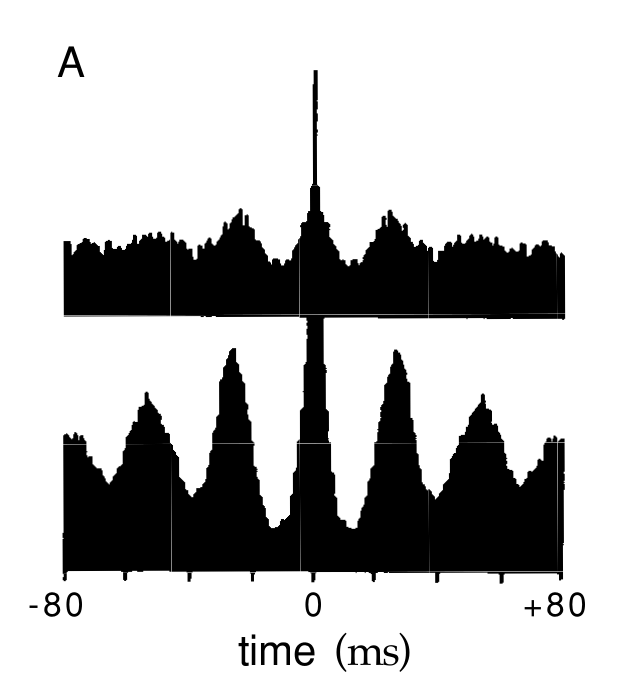
\includegraphics[scale = 0.36]{png/Figure1-12-A.png}
% \end{center}
% \begin{center}
    \label{fig:1.12B} 
    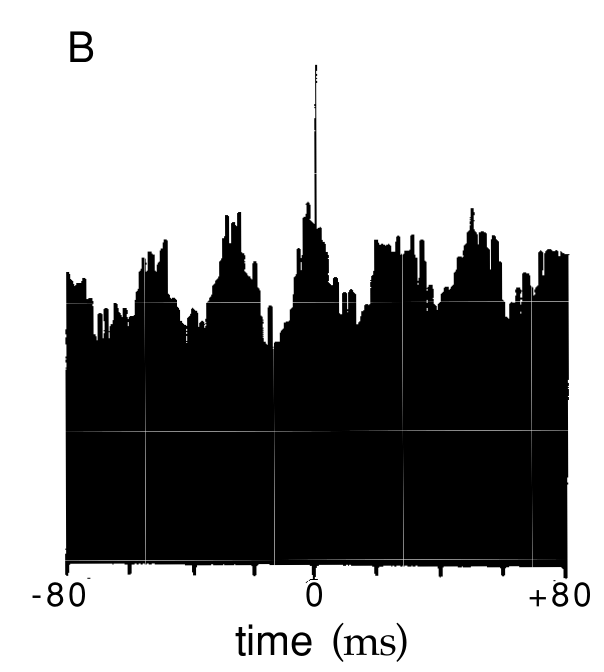
\includegraphics[scale = 0.36]{png/Figure1-12-B.png}\\
\end{center}

\subsection{The Inhomogeneous Poisson Process}
\begin{thm}

The probability density of the inhomogeneous Poisson Process for $n$ spike times is 
    \begin{equation}
    p[t_1, t_2, ..., t_n]=\exp\left(-\int^T_0r(t)dt\right)\prod^n_{i=1}r(t_i),
        \label{equ:1.37}
    \end{equation}
    The spike times are ordered $0\leq t_1 \leq t_2\leq ... \leq t_n \leq T.$
    \begin{proof}
    The probability density for a particular spike sequence with spike times $t_i$ for $i = 1, 2, ..., n$ is obtained from the corresponding probability distribution by multiplying the probability that the spikes occur when they do by the probability that no other spikes occur.We begin by computing the probability that no spikes are generated during the time interval from $t_i$ to $t_{i+1}$ between two adjacent spikes. We determine this by dividing the interval into M bins of size $\Delta t$ and setting $M\Delta t=t_{i+1}-t_i$. We will ultimately take the limit $\Delta t\to 0$. The firing rate during bin $m$ within this interval is $r(t_i+m\Delta t)$. Because the probability of firing a spike in this bin is $r(t_i+m\Delta t)\Delta t$, the probabilities of not firing a spike is $1-r(t_i+m\Delta t)\Delta t$. To have no spikes during the entire interval, we must string together $M$ such bins,  and the probability of this occurring is the product of the individual probabilities, 
            \begin{equation}
            P[\text{no spikes}]=\prod_{m=1}^M(1-r(t_i+m\Delta t)\Delta t).
            \label{equ:1.52}
            \end{equation}
    We evaluate this expression by taking its logarithm,             
            \begin{equation}
            \ln P[\text{no spikes}]=\sum_{m=1}^M\ln(1-r(t_i+m\Delta t)\Delta t),
            \label{equ:1.53}
            \end{equation}
    using the fact that the logarithm of a product is the sum of the logarithms of the multiplied terms. Using the approximation $\ln (1-r(t_i+m\Delta t)\Delta t)\approx -r(t_i+m\Delta t)\Delta t$,  valid for small $\Delta t$, we can simplify this to 
            \begin{equation}
            \ln P[\text{no spikes}]=-\sum_{m=1}^Mr(t_i+m\Delta t)\Delta t.
            \label{equ:1.54}
            \end{equation}
    In the limit $\Delta t \to 0$, the approximation becomes exact and this sum becomes the  integral of $r(t)$ from $t_i$ to $t_{i+1}$, 
            \begin{equation}
            \ln P[\text{no spikes}]=-\int_{t_i}^{t_{i+1}}r(t)dt.
            \label{equ:1.55}
            \end{equation}
    Exponentiating this Equation gives the result we need,             
            \begin{equation}
            P[\text{no spikes}]=\exp\left(-\int_{t_i}^{t_{i+1}}r(t)dt\right).
            \label{equ:1.56}
            \end{equation}
    The probability density $p[t_1, t_2, ..., t_n]$is the product of the densities for the individual spikes and the probabilities of not generating spikes during the interspikde intervals, between time $0$ and the first spike,  and between the time of the last spike and the end of the trial period:            
            \begin{equation}
            \begin{aligned}
            p[t_1, t_2, ...t_n]=\exp\left(-\int_0^{t_1}r(t)dt\right)\exp\left(-\int_{t_n}^Tr(t)dt\right)\times \\  r(t_n)\prod_{i=1}^{n-1}r(t_i)\exp\left(-\int_{t_i}^{t_{i+1}}r(t)dt\right).
            \end{aligned}
            \label{equ:1.57}
            \end{equation}
    The exponentials in this expression all combine because the product of exponentials is the exponential of the sum, so the different integrals in this sum add up to form a single integral:            
            \begin{equation}
                \small
            \begin{aligned}
            &\exp\left(-\int_0^{t_1}r(t)dt)\right)\exp\left(-\int_{t_n}^Tr(t)dt\right)\prod_{i=1}^{n-1}\exp\left(-\int_{t_i}^{t_{i+1}}r(t)dt\right)\\
            &=\exp\left(-\left(\int_0^{t_1}r(t)dt+\sum_{i=1}^{n-1}\int_{t_i}^{t_{i+1}}r(t)dt+\int_{t_n}^Tr(t)dt\right)\right)\\
            &=\exp\left(-\int_0^Tr(t)dt\right) .
            \end{aligned}
            \label{equ:1.58}
            \end{equation}
            Substituting this into Equation \ref{equ:1.57} gives the result in Equation \ref{equ:1.37}
    \end{proof}
\end{thm}

\begin{rem}
The eqution \ref{equ:1.26} is a special case of Equation \ref{equ:1.37}.
\end{rem}

\subsection{The Poisson Spike Generator}

\begin{rul}[\emph{Estimated firing rate}]
    Spike sequences can be simulated by using some estimate of the firing rate, $r_\text{est}(t)$, predicted from knowledge of the stimulus,  to drive a Poisson process.
\end{rul}

\begin{alg}
    The program progresses through time in small steps of size $\Delta t$ and generates, at each time step, a random number $x_{\text{rand}}$ chosen uniformly in the range between $0$ and $1$. If $r_{\text{est}}(t)\Delta t > x_{\text{rand}}$ at that time step, a spike is fired; otherwise it is not.
    % is $r_{est}(t)\Delta t$.
\end{alg}

\begin{alg}
    For a constant firing rate, it is faster to compute spike times $t_i$ for $i=1,2,...,n$ iteratively by generating interspike intervals from an exponential probability density(Equation \ref{equ:1.31}). Thus  we can generate spike times iteratively from the formula $t_{i+1}= t_i-\ln(x_\text{rand}/r)$.
    
 \end{alg}
\begin{rem}
    If $x_\text{rand}$ is uniformly distributed over the range between $0$ and $1$, the negative of its logarithm is exponentially distributed.
\end{rem}
 \begin{alg}[\emph{Spike thinning}]
    The thinning technique requires a bound $r_\text{max}$ on the estimated firing rate such that $r_{\text{est}}(t) \leq r_\text{max}$    at all times. We first generate a spike sequence corresponding to the constant rate $r_{max}$ by iterating the rule $t_{i+1} = t_i - \ln(x_{\text{rand}})/r_\text{max}$. The spike are then thinned by generating another $x_{\text{rand}}$ for each $i$ and removing the spike at time $t_i$ from the train if $r_{\text{est}(t_i)}/r_{\text{max}} < x_{\text{rand}}$. If $r_\text{est}(t_i) / r_{\text{max}} \geq x_{\text{rand}}$, spike $i$ is retained. Thinning corrects for the difference between the estimated timedependent rate and the maximum rate.
    \end{alg} 

\begin{exm}
    The following figures shows an example of a model of an orientation-selective V1 neuron constructed by  Spike thinning. In this model,  the estimated firing rate is determined from the response tuning curve
    \begin{equation}
        r_{est}(t)=f(s(t))=r_{max}\exp\left(-\frac{1}{2}\left(\frac{s(t)-s_{max}}{\sigma_f}\right)^2\right).
        \label{equ:1.38}
    \end{equation}
    % (problem)
\end{exm}

\begin{center}
    \label{fig:1.13A}    
    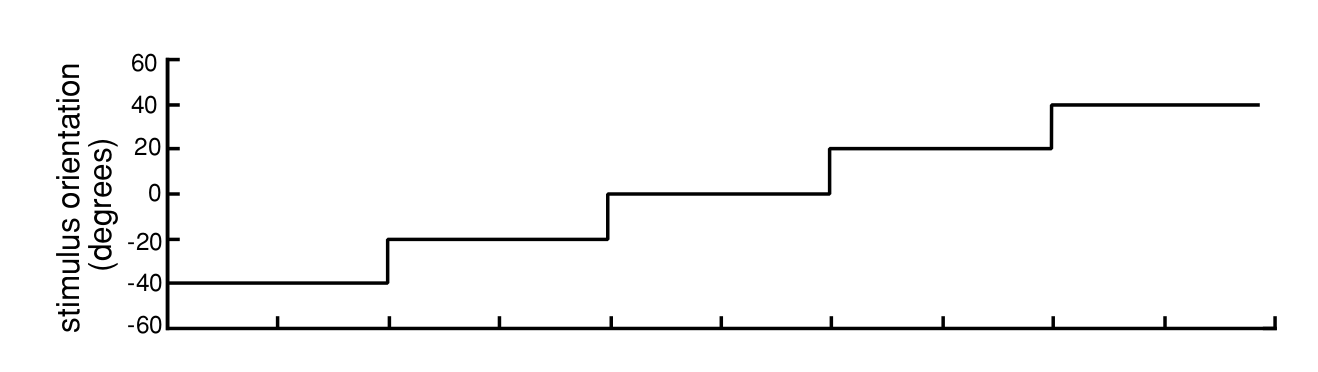
\includegraphics[scale = 0.2]{png/Figure1-13-A.png}\\
\end{center}

\begin{center}
    \label{fig:1.13B}    
    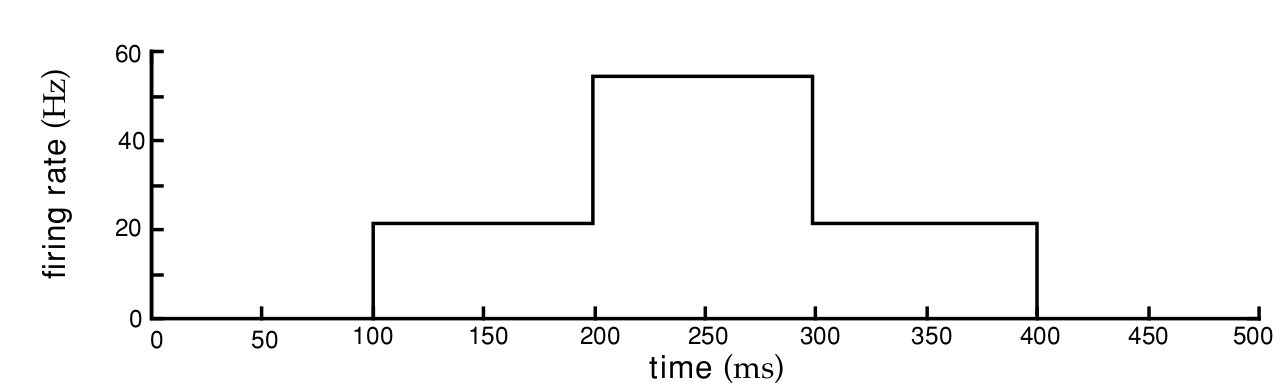
\includegraphics[scale = 0.2]{png/Figure1-13-B.png}\\
\end{center}

\begin{center}
    \label{fig:1.13C}    
    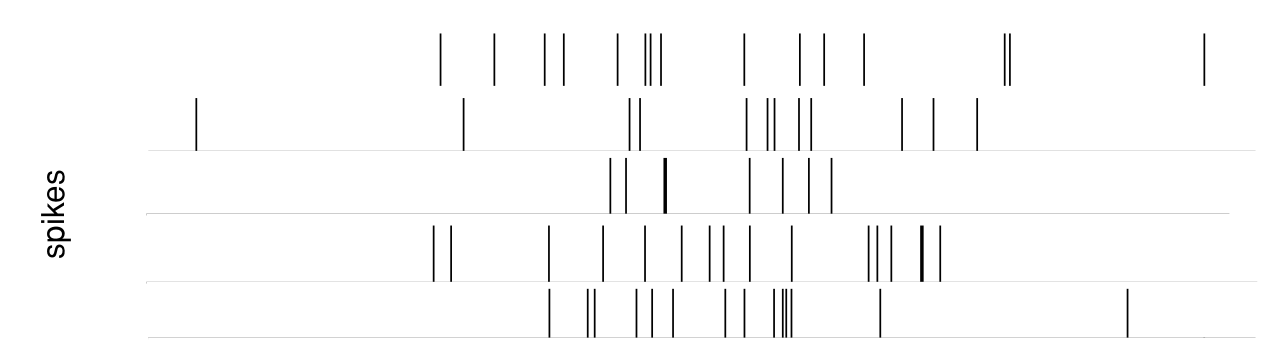
\includegraphics[scale = 0.2]{png/Figure1-13-C.png}\\
\end{center}
This figure Model of an orientation-selective neuron. The orientation angle (top
panel) was increased from an initial value of $-40^\circ$  by $20^\circ $  every $100$ ms. The firing
rate (middle panel) was used to generate spikes (bottom panel) using a Poisson
spike generator. The bottom panel shows spike sequences generated on five different trials.

\subsection{Comparison with Data}
\begin{rem}
    The Poisson process is simple and useful, but does it match data on neural response variability? To address this question,  we examine Fano factors, interspike interval distributions,  and coefficients of variation.
\end{rem}

\begin{prop}
    The Fano factor describes the relationship between the mean spike count over a given interval and the spike-count variance. Mean spike counts $\langle n \rangle $ and variances $\sigma^2_n$ from a wide variety of neuronal recordings have been fitted to the Equation $\sigma^2_n = A\langle n\rangle^B $, and the \emph{multiplier} $A$ and exponent B have been determined. The values of both $A$ and $B$ typically lie between 
    $1.0$ and $1.5.$
\end{prop}

\begin{rem}
    Because the Poisson model predicts $A = B = 1$, this indicates
that the data show a higher degree of variability than the Poisson model
would predict. However, many of these experiments involve anesthetized
animals, and it is known that response variability is higher in anesthetized
than in alert animals.
\end{rem}


\begin{exm}[\emph{comparison of the Fano factor}]
    The following figures shows data for spike-count means and variances extracted
from recordings of MT neurons in alert macaque monkeys using a number of different stimuli. The MT (medial temporal) area is a visual region of the primate cortex where many neurons are sensitive to image motion.
The individual means and variances are scattered in figure A,  but they
cluster around the diagonal which is the Poisson prediction. Similarly,  the
results show A and B values close to $1$,  the Poisson values (figure B).
Of course,  many neural responses cannot be described by Poisson statistics,  but it is reassuring to see a case where the Poisson model seems a
reasonable approximation. As mentioned previously,  when spike trains
are not described very accurately by a Poisson model,  refractory effects
are often the primary reason.
\end{exm}
\begin{center}
    \label{fig:1.14A}    
    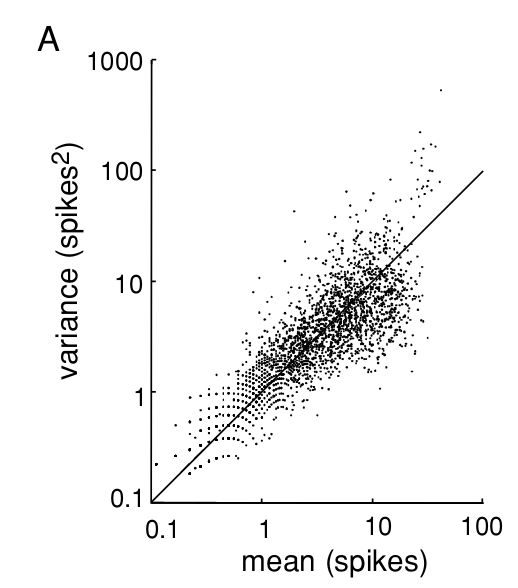
\includegraphics[scale = 0.36]{png/Figure1-14-A.png}\\
\end{center}

\begin{center}
    \label{fig:1.14B}    
    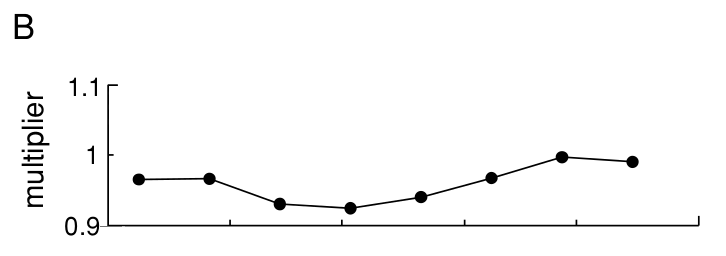
\includegraphics[scale = 0.36]{png/Figure1-14-B.png}\\
\end{center}

\begin{center}
    \label{fig:1.14C}    
    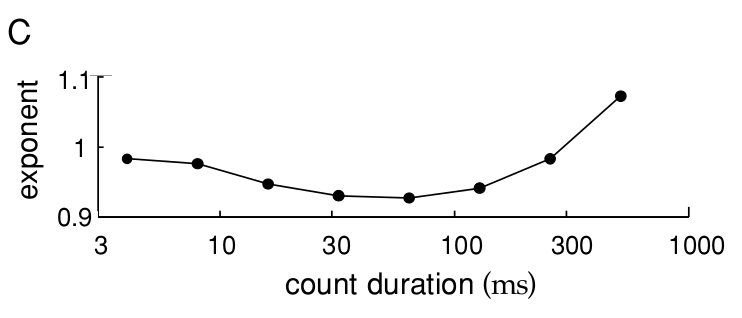
\includegraphics[scale = 0.36]{png/Figure1-14-C.png}\\
\end{center}

\begin{alg}
    Interspike interval distributions are extracted from data as interspike histograms by counting the number of intervals falling in discrete time bins.
\end{alg}

\begin{exm}[\emph{the Poisson model of interspike interval}]
    The following figure presents an example from the responses of a nonbursting cell in area MT of a monkey in response to images consisting of randomly moving dots with a variable amount of coherence imposed on
    their motion (see chapter $3$ for a more detailed description). 
\end{exm}

\begin{center}
    \label{fig:1.15A}    
    % 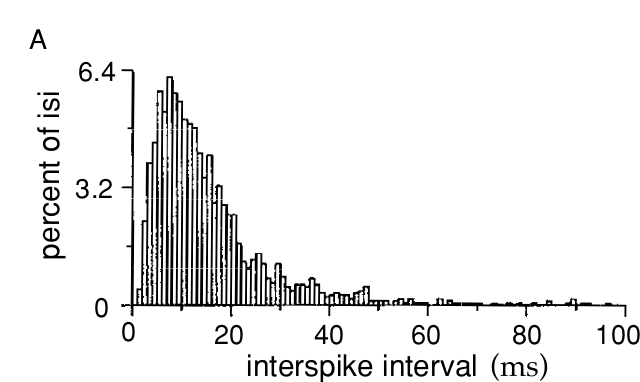
\includegraphics[scale = 0.36]{png/Figure1-15-A.png}\\
    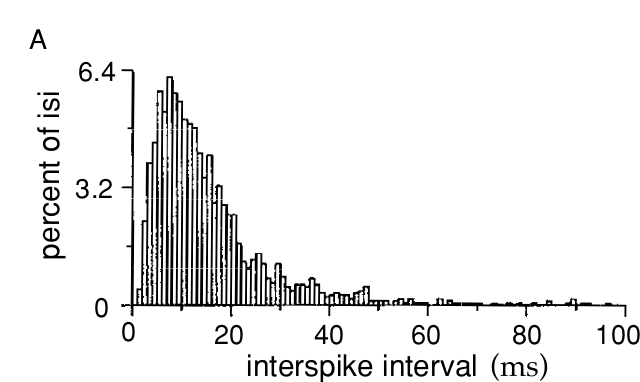
\includegraphics[trim=30 0 0 60,clip,scale = 0.36]{png/Figure1-15-A.png}\\        
\end{center}
For interspike intervals longer than about 10 ms, the shape of this histogram is exponential, in agreement with Equation \ref{equ:1.31}. However, for shorter intervals there is a discrepancy. While the homogeneous Poisson distribution of Equation \ref{equ:1.31} rises for short interspike intervals, the experimental results show a rapid decrease. This is the result of refractoriness making short interspike intervals less likely than the Poisson model would predict.
\begin{rem}
\end{rem}
\begin{prop}
    The data of the Poisson model of interspike interval with a stochastic refractory period can be fitted more accurately by a gamma distribution, 
    \begin{equation}
        p[\tau] = \frac{r(r\tau)^k\exp(-r\tau)}{k!}
        \label{equ:1.39}
    \end{equation}
    with $k>0$, than by the exponential distribution of the Poisson model, which has $k = 0$.
\end{prop}

\begin{exm}[\emph{the Poisson model of interspike interval with a stochastic refractory period}]
    The following figure shows a theoretical histogram obtained by adding a refractory period of variable duration to the Poisson model. Spiking was prohibited during the refractory period,  and then was described once again by a homogeneous Poisson process. The refractory period was randomly chosen from a Gaussian distribution with a mean of $5$ ms and a standard
deviation of $2$ ms (only random draws that generated positive refractory periods were included). The resulting interspike interval distribution of figure \ref{fig:1.15B} agrees quite well with the data.
\end{exm}

\begin{center}
    \label{fig:1.15B}    
    % 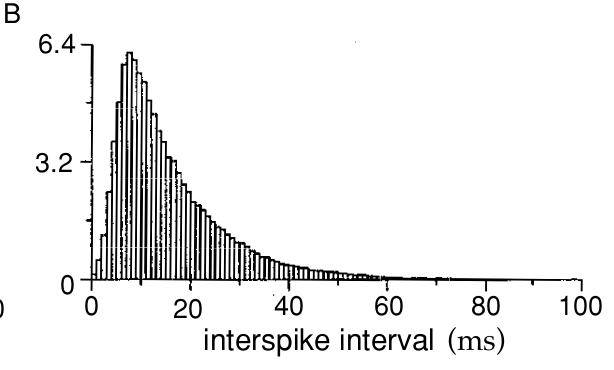
\includegraphics[scale = 0.36]{png/Figure1-15-B.png}\\
    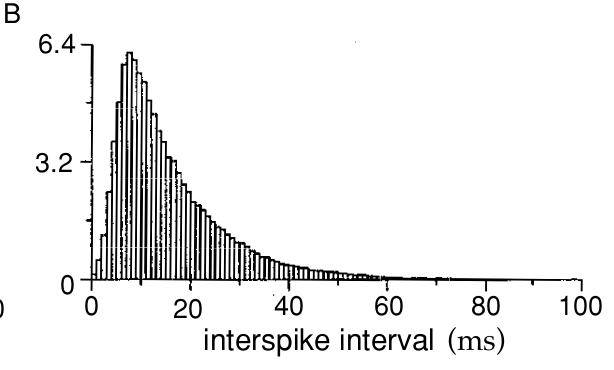
\includegraphics[trim=10 10 30 30,clip,scale = 0.36]{png/Figure1-15-B.png}\\    
\end{center}

\begin{exm}[\emph{comparion of the coefficients of variation}]
    $C_V$ values extracted from the spike trains of neurons recorded in monkeys from area MT and primary visual cortex(V1) are shown in this figure. The data have been divided into groups based on the mean interspike interval,  and the coefficient of variation is plotted as a function of the mean interval,  equivalent to $1/\langle r\rangle$. Except for short mean interspike intervals, the values are near $1$, although they tend to cluster slightly lower than $1$, the Poisson value. The small $C_V$ values for short interspike intervals are due to the refractory period. The solid curve is the prediction of a Poisson  model with refractoriness.
\end{exm}

\begin{center}
    \label{fig:1.16}    
    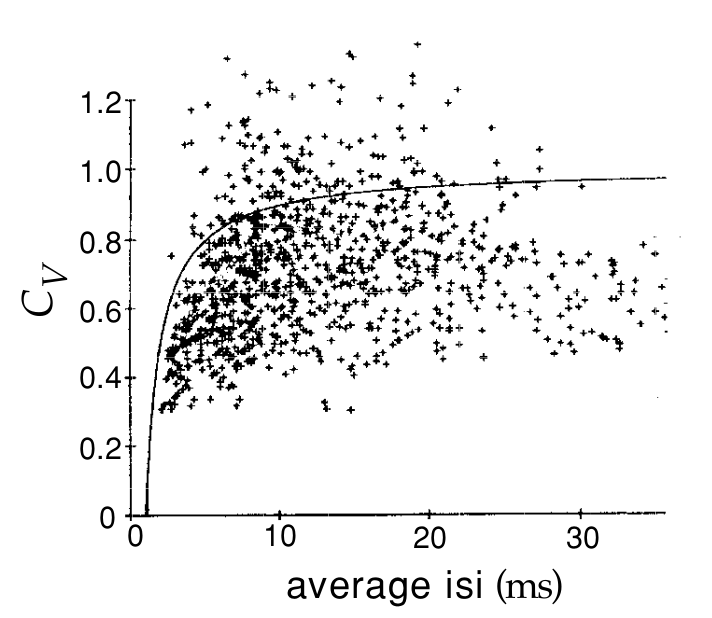
\includegraphics[scale = 0.36]{png/Figure1-16.png}\\
\end{center}

\begin{rem}
    However,  there are cases in which the accuracy in the timing and numbers of spikes fired by a neuron is considerably higher than would be implied by Poisson statistics. 
    Furthermore,  even when it successfully describes data,  the Poisson model does not provide a mechanistic explanation of neuronal response variability.
\end{rem}

\begin{exm}
    The following figure compares the response of V1 cells to constant current injection in vivo and in vitro. The in vitro response is a regular and reproducible spike train(left panel). The same current injection paradigm applied in vivo produces a highly irregular pattern of firing(center panel) similar to the response to a moving bar stimulus(right panel).
\end{exm}

\begin{center}
    \label{fig:1.17}    
    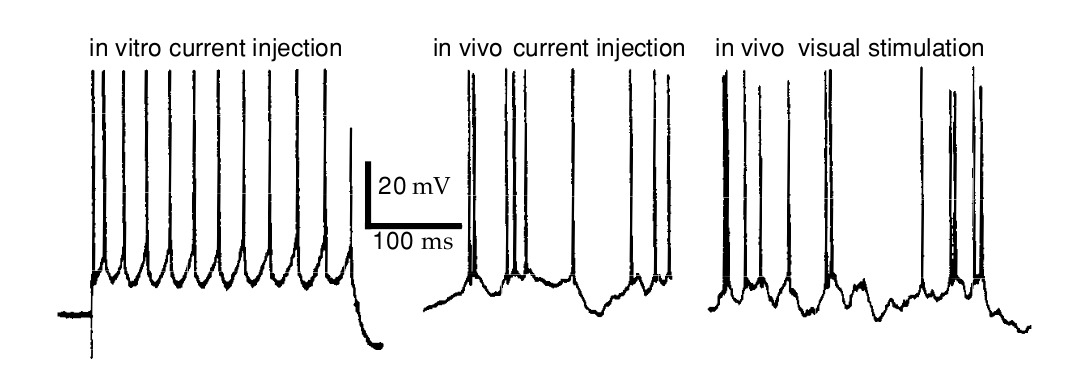
\includegraphics[scale = 0.25]{png/Figure1-17.png}\\
\end{center}
Although some of the basic statistical properties of firing variability may be captured by the Poisson model of spike generation,  the spike generating mechanism itself in real neurons is clearly not responsible for the variability. We explore ideas about possible sources of spike-train variability in chapter $5$.

\begin{rem}
    Some neurons fire action potentials in clusters or bursts of spikes that can not be described by a Poisson process with a fixed rate. Bursting can be included in a Poisson model by allowing the firing rate to fluctuate in order to describe the high rate of firing during a burst. Sometimes the distribution of bursts themselves can be described by a Poisson process (such a doubly stochastic process is called a Cox process).    
\end{rem}





% problem: 推导确认一下
% problem: 那些例子如何修改
% problem: 概念如何改变
% problem: tex规格 ok
% problem: 修改exp  ok
% problem: 具体的排版  ok
% problem: 以及一些公式 ok
% problem: 图像无法正确索引 ok
